\documentclass[a4paper, 10pt, ]{article}

\usepackage[slovak]{babel}





\usepackage[utf8]{inputenc}
\usepackage[T1]{fontenc}

\usepackage[left=4cm,
			right=4cm,
            % left=2.5cm,
			% right=5.5cm,
			top=2.1cm,
			bottom=2.6cm,
			footskip=7.5mm,
			% twoside,
			marginparwidth=3.0cm,
			%showframe,
			]{geometry}

\usepackage{graphicx}
\usepackage[dvipsnames]{xcolor}
% https://en.wikibooks.org/wiki/LaTeX/Colors


% ------------------------------

\usepackage{lmodern}

\usepackage[tt={oldstyle=false,proportional=true,monowidth}]{cfr-lm}

% ------------------------------

\usepackage{amsmath}
\usepackage{amssymb}
\usepackage{amsthm}

\usepackage{booktabs}
\usepackage{multirow}
\usepackage{array}
\usepackage{dcolumn}


\usepackage[singlelinecheck=true]{subfig}


% ------------------------------


\def\naT{\mathsf{T}}

\hyphenpenalty=6000
\tolerance=1000




% ------------------------------


\makeatletter

	\def\@seccntformat#1{\protect\makebox[0pt][r]{\csname the#1\endcsname\hspace{4mm}}}

	\def\cleardoublepage{\clearpage\if@twoside \ifodd\c@page\else
	\hbox{}
	\vspace*{\fill}
	\begin{center}
	\phantom{}
	\end{center}
	\vspace{\fill}
	\thispagestyle{empty}
	\newpage
	\if@twocolumn\hbox{}\newpage\fi\fi\fi}

	\newcommand\figcaption{\def\@captype{figure}\caption}
	\newcommand\tabcaption{\def\@captype{table}\caption}

\makeatother


% ------------------------------




\usepackage{fancyhdr}
\fancypagestyle{plain}{%
\fancyhf{} % clear all header and footer fields
\fancyfoot[C]{\sffamily {\bfseries \thepage}\ | {\scriptsize\oznacenieCasti}}
\renewcommand{\headrulewidth}{0pt}
\renewcommand{\footrulewidth}{0pt}}
\pagestyle{plain}


% ------------------------------


\usepackage{titlesec}
\titleformat{\paragraph}[hang]{\sffamily  \bfseries}{}{0pt}{}
\titlespacing*{\paragraph}{0mm}{3mm}{1mm}
\titlespacing*{\subparagraph}{0mm}{3mm}{1mm}

\titleformat*{\section}{\sffamily\Large\bfseries}
\titleformat*{\subsection}{\sffamily\large\bfseries}
\titleformat*{\subsubsection}{\sffamily\normalsize\bfseries}






% ------------------------------

\PassOptionsToPackage{hyphens}{url}
\usepackage[pdfauthor={},
			pdftitle={},
			pdfsubject={},
			pdfkeywords={},
			% hidelinks,
			colorlinks=false,
			breaklinks,
			]{hyperref}


% ------------------------------


\graphicspath{%
{../fig_standalone/}%
{../../PY/fig/}%
{../../PY/jupynotex/fig/}%
{../../ML/fig/}%
{./fig/}%
}



% ------------------------------

\usepackage{enumitem}

\usepackage{lettrine}

% ------------------------------


\usepackage{microtype}


% ------------------------------

\usepackage[titles]{tocloft}

\setlength{\cftsecindent}{-12mm}
\setlength{\cftsecnumwidth}{12mm}
\renewcommand{\cftsecpresnum}{\hfill}
\renewcommand{\cftsecaftersnum}{\hspace{4mm}}

\setlength{\cftsubsecindent}{-12mm}
\setlength{\cftsubsecnumwidth}{16mm} % 12 + 4
\renewcommand{\cftsubsecpresnum}{\hfill}
\renewcommand{\cftsubsecaftersnum}{\hspace{8mm}} % 4 + 4 mm

\setlength{\cftsubsubsecindent}{-12mm}
\setlength{\cftsubsubsecnumwidth}{20mm} % 12 + 4 + 4
\renewcommand{\cftsubsubsecpresnum}{\hfill}
\renewcommand{\cftsubsubsecaftersnum}{\hspace{12mm}} % 4 + 4 + 4 mm

\renewcommand{\cftsecpagefont}{\lstyle \bfseries}
\renewcommand{\cftsubsecpagefont}{\lstyle}
\renewcommand{\cftsubsubsecpagefont}{\lstyle}



\setlength{\cftparaindent}{-16mm}
\setlength{\cftparanumwidth}{28mm} % 16 + 4 + 4 + 4
\renewcommand{\cftparapresnum}{\hfill}
\renewcommand{\cftparaaftersnum}{\hspace{16mm}} % 4 + 4 + 4 + 4 mm








% ------------------------------

\usepackage{listings}



\renewcommand{\lstlistingname}{Výpis kódu}
\renewcommand{\lstlistlistingname}{Výpisy kódu}




%New colors defined below
\definecolor{codegreen}{rgb}{0,0.6,0}
\definecolor{codegray}{rgb}{0.5,0.5,0.5}
\definecolor{codepurple}{rgb}{0.58,0,0.82}
\definecolor{backcolour}{rgb}{0.95,0.95,0.95}

%Code listing style named "mystyle"
\lstdefinestyle{mystyle}{
  backgroundcolor=\color{backcolour},
  commentstyle=\fontfamily{lmtt}\fontsize{8.5pt}{8.75pt}\selectfont\color{codegreen},
  keywordstyle=\fontfamily{lmtt}\fontsize{8.5pt}{8.75pt}\selectfont\bfseries\color{Blue},
  stringstyle=\fontfamily{lmtt}\fontsize{8.5pt}{8.75pt}\selectfont\color{codepurple},
  basicstyle=\fontfamily{lmtt}\fontsize{8.5pt}{8.75pt}\selectfont,
  breakatwhitespace=false,
  breaklines=true,
  captionpos=t,
  keepspaces=true,
  numbers=left,
  numbersep=4mm,
  numberstyle=\fontfamily{lmtt}\fontsize{8.5pt}{8.75pt}\selectfont\color{lightgray},
  showspaces=false,
  showstringspaces=false,
  showtabs=false,
  tabsize=2,
  % xleftmargin=10pt,
  framesep=10pt,
  language=Python,
  escapechar=|,
}


\lstset{
    inputencoding=utf8,
    extendedchars=true,
    literate=%
    {á}{{\'a}}1
    {č}{{\v{c}}}1
    {ď}{{\v{d}}}1
    {é}{{\'e}}1
    {ě}{{\v{e}}}1
    {í}{{\'i}}1
    {ň}{{\v{n}}}1
    {ó}{{\'o}}1
    {ř}{{\v{r}}}1
    {š}{{\v{s}}}1
    {ť}{{\v{t}}}1
    {ú}{{\'u}}1
    {ů}{{\r{u}}}1
    {ý}{{\'y}}1
    {ž}{{\v{z}}}1
    {Á}{{\'A}}1
    {Č}{{\v{C}}}1
    {Ď}{{\v{D}}}1
    {É}{{\'E}}1
    {Ě}{{\v{E}}}1
    {Í}{{\'I}}1
    {Ň}{{\v{N}}}1
    {Ó}{{\'O}}1
    {Ř}{{\v{R}}}1
    {Š}{{\v{S}}}1
    {Ť}{{\v{T}}}1
    {Ú}{{\'U}}1
    {Ů}{{\r{U}}}1
    {Ý}{{\'Y}}1
    {Ž}{{\v{Z}}}1
    {ô}{{\^{o}}}1
}


% ------------------------------


\usepackage{caption}

\DeclareCaptionFormat{odsadene}{\protect\makebox[0pt][r]{#1#2\hspace{4mm}}#3\par}
\DeclareCaptionLabelSeparator{lendvojbodka}{:}
% \DeclareCaptionFont{lightgray}{\color{lightgray}}
\DeclareCaptionFont{lightgray}{\fontfamily{lmtt}\fontsize{8.5pt}{8.75pt}\selectfont\color{lightgray}}

\captionsetup[lstlisting]{format=odsadene, labelsep=lendvojbodka, justification=raggedright, singlelinecheck=false, labelfont={sf, lightgray},}


% ------------------------------





% ------------------------------

\usepackage[backend=biber,
            style=numeric,
            sorting=none,
            ]{biblatex}
\DeclareSourcemap{
    \maps[datatype=bibtex]{
        \map{
        \step[fieldset=note, null]
        }
        \map{
        \step[fieldset=file, null]
        }        
        % \map{
        % \step[fieldset=url, null]        
        % }
        \map{
        \step[fieldset=eprint, null]
        }
    }
}


\addbibresource{E:/_CurrentContent/01_work_repo/bibLaTeXDB/bibLaTeXDB.bib} % nonpublic data





\def\oznacenieCasti{AR01 - LS2022}





\begin{document}

\lstset{style=mystyle}




\fontsize{12pt}{22pt}\selectfont

\centerline{\textsf{Adaptívne riadenie} \hfill \textsf{\oznacenieCasti}}

\fontsize{18pt}{22pt}\selectfont





\begin{flushleft}
	\textbf{\textsf{Veľmi stručný prehľad Adaptívneho riadenia}}
\end{flushleft}





\normalsize

\bigskip

{\hypersetup{hidelinks}

\tableofcontents

}

\bigskip

\vspace{18pt}




\section{História a nedávna história}




\lettrine[lines=3, nindent=0pt]N{ázvy} \emph{Adaptívny systém} a \emph{Adaptívne riadenie} boli v publikáciách prvý krát použité okolo roku 1950. Motiváciou pre vývoj adaptívnych regulátorov bol návrh autopilota pre vysokovýkonné experimentálne lietadlá na začiatku 50-tych rokov.

Lietadlo operuje vo veľkom rozsahu rýchlostí a výšok. Komplexná dynamika lietadla môže byť pre daný pracovný bod (rýchlosť, výška) aproximovaná lineárnym modelom v tvare
\begin{subequations}
\begin{align}
	\dot{x}(t) &= A x(t) + B u(t)  \\
	y(t) &= C x(t) + D u(t)
\end{align}
\end{subequations}
pričom $A$, $B$, $C$ a $D$ sú funkciou pracovného bodu, ktorý sa mení v čase (teda $A$, $B$, $C$ a $D$ sú funkciou času).

Zjednodušene, tá istá výchylka „smerovky“ (alebo kormidla na lodi) spôsobí pri rôznych rýchlostiach iný moment sily (ktorý otáča lietadlo alebo loď). Teda mení sa parameter riadeného systému, ktorý môže byť opísaný napríklad prenosovou funkciou, ktorej vstupom je výchylka kormidla a výstupom je kurz (natočenie) lode.

\bigskip

\noindent
Toľko veľmi stručné zhrnutie inak veľmi rozsiahlej histórie Adaptívneho riadenia.

\bigskip

\noindent
Ako príklad súčasného/nedávneho využitia Adaptívneho riadenia možno uviesť opäť systémy riadenia letu. V správe \emph{The Impact of Control Technology, T. Samad and A.M. Annaswamy (eds.), IEEE Control Systems Society, 2011, available at www.ieeecss.org.} je uvedený takýto príklad.

Názvom \emph{The Joint Direct Attack Munition} sa označuje navádzací systém, ktorý konvertuje nenavádzané bomby na \emph{smart} muníciu schopnú činnosti v~každom počasí. V tomto systéme sa uplatňuje robustné a adaptívne riadenie. Navzájom sa dopĺňajú a~kombinujú.

Tento príklad uvádzame najmä preto, aby sme čitateľa upozornili na uvedenú správu. Medzičasom (2014) je dostupná aj druhá edícia tejto správy, dostupné na: \url{http://ieeecss.org/impact-control-technology-2nd-edition}.












\begin{figure}[!t]
	\centering
	\makebox[\textwidth][c]{%
		\subfloat[Základá schéma adaptívneho riadenia]{%
			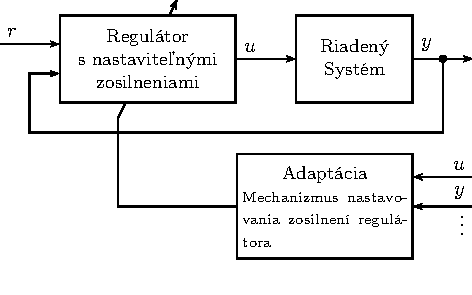
\includegraphics{Obr_ZaklSchemaAR_standalone.pdf} \medskip
		}
		\quad
		\subfloat[Schéma Gain Scheduling]{%
			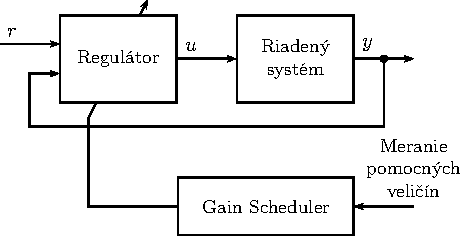
\includegraphics{Obr_SchemaGS_standalone.pdf}
		}
	}
	\figcaption{Základá schéma adaptívneho riadenia a schéma Gain Scheduling}
	\label{Základá schéma adaptívneho riadenia a schéma Gain Scheduling}
\end{figure}








\bigskip

\noindent
Autor si na začiatku roka 2022 uvedomuje možnú zmätenosť čitateľa ak sa za súčasnosť, či nedávnu minulosť označujú roky 2011, prípadne 2014. Ide však o obdobie, keď vznikal tento učebný text. Adaptívne riadenie, ako pojem, sa možno vytráca, avšak princípy, najmä v spojení s identifikáciou systémov vo všeobecnosti, sú viac ako aktuálne. Nájdeme ich prezlečené alebo zaradené pod pojmy ako je strojové učenie (machine learning), spracovanie signálov (signal processing) alebo priebežná identifikácia systémov.

Podobne, ak sa čitateľovi zdá odporúčaná literatúra staršieho dáta, nech má na pamäti, že ide o relatívne novinky v čase poslednej rozsiahlejšej aktualizácie tohto učebného materiálu -- predovšetkým kniha \cite{IF06} z roku 2006. Ostatné sa dajú považovať za klasické učebnice tohto predmete a do popredia tu dávame knihu \cite{IS96} najmä pre skutočnosť, že je voľne dostupná tu: \url{https://viterbi-web.usc.edu/~ioannou/RobustAdaptiveBook95pdf/Robust_Adaptive_Control.pdf}.












\section{Schémy Adaptívneho riadenia}


Túto časť možno chápať aj ako veľmi stručné\footnote{Všetko je tu akosi veľmi stručné\ldots} rozdelenie Adaptívneho riadenia.


\subsection{Základná schéma AR}

Priebeh výstupnej veličiny obsahuje informáciu o stave $x$ systému a~o~parametroch systému. Preto by nejaký sofistikovaný spätnoväzbový riadiaci systém mal byť schopný vysporiadať sa so zmenami v riadenom systéme a zabezpečiť dosiahnutie požadovaného cieľa riadenia. Tieto myšlienky viedli k návrhu spätnoväzbovej štruktúry riadenia, ktorá je základom adaptívneho riadenia.

V~štandardnom regulačnom obvode (v~uzavretom regulačnom obvode -- URO) je použitý regulátor, ktorého parametre (zosilnenia) je možné meniť (aj v~počas činnosti). K~uzavretému obvodu je pridaný mechanizmus pre nastavovanie zosilnení regulátora. Podľa spôsobu určenia zmeny zosilnení regulátora (v reakcii na zmenu parametrov riadeného systému a~teda na zmenu v~dynamike sústavy a porúch) sa odlišujú rôzne typy schém adaptívneho riadenia.

\subsubsection{Robustné riadenie}

Pre vysporiadanie sa so zmenami parametrov riadeného systému môže byť navrhnutý aj regulátor s konštantnými zosilneniami --- týmto sa zaoberá \emph{Robustné riadenie}. Regulátor navrhnutý metódami robustného riadenia sa však nepovažuje za adaptívny regulátor aj keď dokáže zvládnuť zmenu parametrov sústavy.



\subsection{Gain Scheduling}

Uvažujme, že v pracovnom bode $i$ sú parametre modelu lietadla $A_i$, $B_i$, $C_i$ a $D_i$ známe. Pre daný pracovný bod teda vieme určiť regulátor, ktorý zabezpečí vyšpecifikované ciele. Zosilnenia takého regulátora označme $\Theta_i$. Pri uvažovaní viacerých pracovných bodov máme množinu zosilnení: $\Theta_1,\ldots, \Theta_i,\ldots, \Theta_N$, kde $N$ je počet uvažovaných pracovných bodov.

Po detegovaní pracovného bodu sa na regulátore nastavia (prepnú) príslušné zosilnenia (parametre regulátora). Tento spôsob adaptácie sa nazýva \uv{Prepínanie parametrov regulátora} --- \emph{Gain Scheduling} (GS).

Prechody medzi pracovnými bodmi sa riešia napríklad interpoláciou určených zosilnení alebo zvýšením počtu uvažovaných (detegovaných) pracovných bodov.

Dvomi prvkami, ktoré sú charakteristické pre GS sú \emph{Look-up Table} (Vyhľadávacia tabuľka -- tabuľka, v~ktorej sa vyhľadávajú príslušné zosilnenia) a \emph{meranie pomocných veličín}, takých ktoré sú vo vhodnom vzťahu s pracovným bodom. Na základe merania pomocných veličín sa rozhoduje (určuje), v~ktorom pracovnom bode sústava operuje a podľa toho sa vyhľadajú a prepnú príslušné zosilnenia regulátora.

Výhodou GS je, že zosilnenia regulátora sa menia okamžite po detegovaní nového pracovného bodu. Výhodou je teda rýchlosť nájdenia teoreticky správnych parametrov regulátora. Časté a rýchle zmeny zosilnení regulátora však môžu viesť k nestabilite celého systému. Preto sa pridávajú obmedzenia pre frekvenciu prepínania.

Nevýhodou je, že mechanizmus prepínania a zosilnenia sú určené vopred (off-line) a teda kompenzácia prípadnej odchýlky od predpokladaného správania nie je možná. Nepredvídateľné zmeny dynamiky sústavy môžu viesť k zhoršeniu kvality riadenia alebo až k~úplnému zlyhaniu. Ďalšou nevýhodou sú vysoké náklady na návrh a~najmä na implementáciu, ktoré narastajú so zvyšujúcim sa počtom pracovných bodov.


















\begin{figure}[!t]
	\centering

	\vspace{-3mm}

	\makebox[\textwidth][c]{%
		\subfloat[Priame adaptívne riadenie]{
		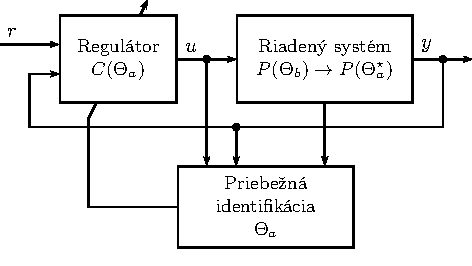
\includegraphics{Obr_SchemaPAR_standalone.pdf}
		}
		\quad
		\subfloat[Nepriame adaptívne riadenie]{
		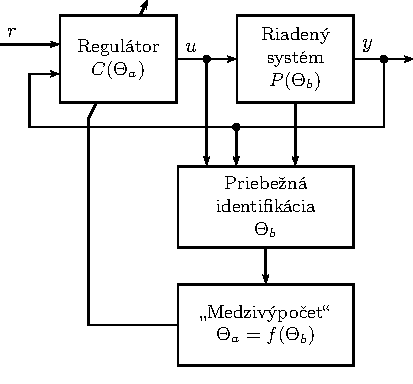
\includegraphics{Obr_SchemaNAR_standalone.pdf}
		}
	}
	\caption{Principiálne schémy priameho a nepriameho adaptívneho riadenia}
	\label{Principiálne schémy priameho a nepriameho adaptívneho riadenia}
\end{figure}



\subsection{Priame a nepriame AR}

Vo všeobecnosti, adaptívny regulátor sa skladá z on-line estimátora (priebežná identifikácia) neznámych parametrov a zákona riadenia (algoritmus riadenia, regulátor). Zákon riadenia je motivovaný prípadom keď hodnoty parametrov sústavy sú známe, avšak konštantné zosilnenia sú nahradené časovo premenlivými.

Spôsob akým je on-line estimátor, nazývaný \emph{Zákon adaptácie}, skombinovaný so zákonom riadenia určuje jeden z dvoch prístupov v~adaptívnom riadení: Priame adaptívne riadenie a Nepriame adaptívne riadenie.

Pri nepriamom adaptívnom riadení sa priebežne identifikujú parametre uvažovaného modelu systému a~následne sú tieto použité pri výpočte zosilnení zákona riadenia. Predpokladá sa pri tom, že identifikované parametre systému sú istotne ekvivalentné so skutočnými parametrami systému. Medzivýpočet potrebný pre výpočet parametrov zákona riadenia charakterizuje nepriame adaptívne riadenie.

Pri priamom adaptívnom riadení je model systému parametrizovaný z hľadiska parametrov zákona riadenia. Rovnica modelu systému je vyjadrená tak, že obsahuje ideálne parametre zákona riadenia. Práve tieto parametre sú priebežne identifikované (pretože ideálne parametre sú neznáme) -- adaptované. Výstupom priebežnej identifikácie (zákona adaptácie) sú teda priamo parametre zákona riadenia. Nie je potrebný medzivýpočet ako v prípade nepriameho adaptívneho riadenia.



\bibliography{../misc_LaTeX/Bib_KurzAR}{}
\bibliographystyle{plain}



\section{Otázky a úlohy}

\begin{enumerate}[leftmargin=0pt, labelsep=4mm, itemsep=0pt]
	\item Nakreslite základnú schému adaptívneho riadenia.
	\item Nakreslite schému Gain Scheduling.
	\item Nakreslite schému priameho adaptívneho riadenia.
	\item Nakreslite schému nepriameho adaptívneho riadenia.
	\item Vysvetlite rozdiel medzi priamym a nepriamym adaptívnym riadením.
\end{enumerate}




\end{document}
